\section{Tensor Notation}
\begin{table}[H]
    \centering
    \caption{Different Rank Tensors}
    \begin{tabular}{cccc}
        \toprule
        Rank & Name & Notation & Example \\
        \midrule
        0 & Scalar & $T$ & Temperature, Pressure, Volume \\
        1 & Vector & $T_i$ & Force, Velocity, Vorticity \\
        2 & Matrix & $T_{ij}$ & Stress, Strain, Rate of Deformation \\
        3 & Third Order Tensor & $T_{ijk}$ & ... \\
        4 & Fourth Order Tensor & $T_{ijkl}$ & ... \\
        ... & ... & ... & ... \\
        \bottomrule
    \end{tabular}
\end{table}

\subsection{Einstein Summation Convention}
The Einstein Summation Convention is a shorthand notation for writing out long sums. It is used to simplify the notation of tensor operations. The convention is as follows:
\begin{itemize}
    \item If an index appears more than once in a term, it is a dummy index. It is summed over.
    \item If an index appears once in a term, it is a free index. The number of free indices is the rank of the tensor.
\end{itemize}

\subsubsection{Examples}
\subsubsubsection{Example 1}

Consider,
\begin{align*}
    A_{ij} &=
    \begin{bmatrix}
        A_{11} & A_{12} & A_{13} \\
        A_{21} & A_{22} & A_{23} \\
        A_{31} & A_{32} & A_{33}
    \end{bmatrix} 
\end{align*}
There are two free indices, $i$ and $j$. The rank of the tensor is 2. \\

\subsubsubsection{Example 2}

Consider, 
\begin{align*}
    \partial_i u_{ij} &= \begin{bmatrix}
        \partial_1 u_{11} + \partial_2 u_{12} + \partial_3 u_{13} \\
        \partial_1 u_{21} + \partial_2 u_{22} + \partial_3 u_{23} \\
        \partial_1 u_{31} + \partial_2 u_{32} + \partial_3 u_{33}
    \end{bmatrix}
\end{align*}
There is one free index, $j$, and one dummy index, $i$. The rank of the tensor is 1.

\subsection{Kronecker Delta}
The Kronecker Delta is a mathematical operator that is used to represent the identity matrix. It is defined as:
\begin{align*}
    \delta_{ij} &= 
    \begin{cases}
        1 & \text{if } i = j \\
        0 & \text{if } i \neq j
    \end{cases} \\
    &=
    \begin{bmatrix}
        1 & 0 & 0 \\
        0 & 1 & 0 \\
        0 & 0 & 1
    \end{bmatrix}
\end{align*}

\subsubsection{Properties (in 3D)}
\begin{itemize}
    \item $\delta_{ij} = \delta_{ji}$
    \item $\delta_{ij}A_{jk} = A_{ik}$
    \item $\delta_{ij}\delta_{jk} = \delta_{ik}$
    \item $\delta_{ij}\delta_{ij} = \delta_{ii} = 3$
    \item $a_{ij} \delta_{ij} = \delta_{ij} a_{ij} = a_{ii}$
\end{itemize}

\subsection{Levi-Civita Symbol}
The Levi-Civita Symbol is a mathematical operator that is used to represent the permutation of indices. It is defined as:
\begin{align*}
    \varepsilon_{ijk} &= 
    \begin{cases}
        1 & \text{if } ijk \text{ is an even permutation of } 123 \\
        -1 & \text{if } ijk \text{ is an odd permutation of } 123 \\
        0 & \text{if any two indices are equal}
    \end{cases}
\end{align*}
\begin{figure}[H]
    \centering
    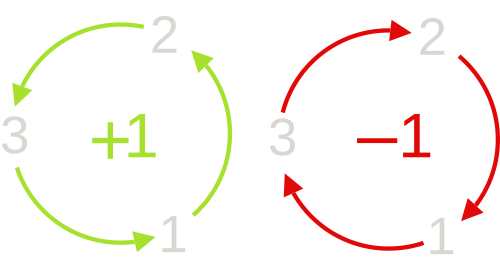
\includegraphics[width=0.5\linewidth]{Section/Figures/levi-civita-cycle-permutation.png}
    \caption{Levi-Civita Even and Odd Permutations}
\end{figure}

For example,
\begin{align*}
    \varepsilon_{123} &= 1 \\
    \varepsilon_{231} &= 1 \\
    \varepsilon_{312} &= 1 \\
    \varepsilon_{132} &= -1 \\
    \varepsilon_{213} &= -1 \\
    \varepsilon_{321} &= -1 \\
    \varepsilon_{122} &= 0 \\
    \varepsilon_{113} &= 0 \\
    \varepsilon_{111} &= 0 \\
\end{align*}

Since this is a third order tensor, there are 27 components. From these, 3 of these components are $+1$, 3 are $-1$, and 21 are $0$.

\subsubsection{Properties (in 3D)}
\begin{itemize}
    \item $\varepsilon_{ijk} = \varepsilon_{jki} = \varepsilon_{kij}$
    \item $\varepsilon_{ijk}\varepsilon_{ijk} = 6$
    \item $\varepsilon_{ijk}\varepsilon_{imn} = \delta_{jm}\delta_{kn} - \delta_{jn}\delta_{km}$
    \item $\varepsilon_{ijk} = -\varepsilon_{ikj}$
    \item $a_{ij}\varepsilon_{ijk} = \varepsilon_{ijk}a_{ij}$
\end{itemize}

\subsection{Vector and Tensor Operations}
\subsubsection{Multiplication of a Vector by a Scalar}
\begin{align*}
    \alpha \vec{A} &= \vec{B} \\
    \alpha A_i &= B_i
\end{align*}

\subsubsection{Dot Product of Two Vectors}
\begin{align*}
    \vec{A} \cdot \vec{B} &= C \\
    A_i B_i &= C
\end{align*}

\subsubsection{Cross Product of Two Vectors}
\begin{align*}
    \vec{A} \cross \vec{B} &= \vec{C} \\
    \varepsilon_{ijk}A_jB_k &= C_i 
\end{align*}

\subsubsection{Dot Product of Two Tensors (Tensor Product)}
\begin{align*}
    %use \otimes
    A \otimes B &= A_{ij}B_{jk}= C_{ik}
\end{align*}

\subsubsection{Double Dot Product of Two Tensors}
\begin{align*}
    A : B &= A_{ij}B_{ij} = C
\end{align*}
A property of the double dot product is that it is commutative, 
\begin{align*}
    A : B &= B : A
\end{align*}

\subsubsection{Nabla Operator}
The Nabla operator is a vector differential operator. It is defined as:
\begin{align*}
    \nabla &= \frac{\partial}{\partial x_i} = \partial_{i} 
\end{align*}
In vector notation,
\begin{align*}
    \nabla &= \begin{bmatrix}
        \frac{\partial}{\partial x_1} \\
        \frac{\partial}{\partial x_2} \\
        \frac{\partial}{\partial x_3}
    \end{bmatrix}
\end{align*}

\subsubsubsection{Gradient of a Scalar}
The gradient of a scalar is a vector. It is defined as:
\begin{align*}
    \nabla T &= \frac{\partial T}{\partial x_i} = \partial_{i} T
\end{align*}

\subsubsubsection{Gradient of a Vector}
The gradient of a vector is a tensor. It is defined as:
\begin{align*}
    \nabla \vec{A} &= \frac{\partial A_j}{\partial x_i} = \partial_{i} A_j \\
    &= \begin{bmatrix}
        \partial_{1} A_1 & \partial_{1} A_2 & \partial_{1} A_3 \\
        \partial_{2} A_1 & \partial_{2} A_2 & \partial_{2} A_3 \\
        \partial_{3} A_1 & \partial_{3} A_2 & \partial_{3} A_3
    \end{bmatrix}
\end{align*}

\subsubsubsection{Divergence of a Vector}
The divergence of a vector is a scalar. It is defined as:
\begin{align*}
    \nabla \cdot \vec{A} &= \frac{\partial A_i}{\partial x_i} = \partial_{i} A_i = \Div(\vec{A}) \\
    &= \partial_{1} A_1 + \partial_{2} A_2 + \partial_{3} A_3 \\
    &= C
\end{align*}

\subsubsubsection{Divergence of a Tensor}
The divergence of a rank 2 tensor is a vector. It is defined as:
\begin{align*}
    \nabla \cdot A &= \frac{\partial A_{ij}}{\partial x_i} = \partial_{i} A_{ij} \\
    &= \begin{bmatrix}
        \partial_{1} A_{11} + \partial_{2} A_{21} + \partial_{3} A_{31} \\
        \partial_{1} A_{12} + \partial_{2} A_{22} + \partial_{3} A_{32} \\
        \partial_{1} A_{13} + \partial_{2} A_{23} + \partial_{3} A_{33}
    \end{bmatrix}
\end{align*}

\subsubsubsection{Curl of a Vector}
The curl of a vector is a vector. It is defined as:
\begin{align*}
    \nabla \cross \vec{A} &= \varepsilon_{ijk}\partial_{j} A_k = \Curl(\vec{A}) \\
    &= \begin{bmatrix}
        \partial_{2} A_3 - \partial_{3} A_2 \\
        \partial_{3} A_1 - \partial_{1} A_3 \\
        \partial_{1} A_2 - \partial_{2} A_1
    \end{bmatrix}
\end{align*}

\subsubsubsection{Laplace of a Scalar}
The Laplace of a scalar is a scalar. It is defined as:
\begin{align*}
    \nabla^2 \phi &= \Div(\Grad(\phi)) = \nabla \cdot (\nabla \phi) \\
    &= \partial_{i} (\partial_{i} \phi)  = \partial_{i} \partial_{i} \phi \\
    &= \partial_{1} \partial_{1} \phi + \partial_{2} \partial_{2} \phi + \partial_{3} \partial_{3} \phi
\end{align*}

\subsubsubsection{Laplace of a Vector}
The Laplace of a vector is a vector. It is defined as:
\begin{align*}
    \nabla^2 \vec{A} &= \Div(\Grad(\vec{A})) = \nabla \cdot (\nabla \vec{A}) \\
    &= \partial_{i} (\partial_{i} A_j)  = \partial_{i} \partial_{i} A_j \\
    &= \begin{bmatrix}
        \partial_{1} \partial_{1} A_1 + \partial_{2} \partial_{2} A_1 + \partial_{3} \partial_{3} A_1 \\
        \partial_{1} \partial_{1} A_2 + \partial_{2} \partial_{2} A_2 + \partial_{3} \partial_{3} A_2 \\
        \partial_{1} \partial_{1} A_3 + \partial_{2} \partial_{2} A_3 + \partial_{3} \partial_{3} A_3
    \end{bmatrix}
\end{align*}

\subsubsubsection{Vector Outer Product (Dyadic Product)}
The vector outer product is a rank 2 tensor. It is defined as:
\begin{align*}
    \vec{A} \vec{B} &= \vec{A} \vec{B}^T  = \begin{bmatrix} a_1 \\ a_2 \\ a_3 \end{bmatrix} [b_1 \quad b_2 \quad b_3] \\
    &= \begin{bmatrix}
        a_1 b_1 & a_1 b_2 & a_1 b_3 \\
        a_2 b_1 & a_2 b_2 & a_2 b_3 \\
        a_3 b_1 & a_3 b_2 & a_3 b_3
    \end{bmatrix} \\
    &= A_i B_j = C_{ij}
\end{align*}

\subsection{Summary of Tensor Operations}
\begin{table}[H]
    \centering
    \caption{Summary of Tensor Operations}
    \begin{tabular}{p{0.5 \textwidth}cc}
        \toprule
        Description & Vector Notation & Einstein Notation \\
        \midrule
        Multiplication of a Vector by a Scalar & $\alpha \vec{A}$ & $\alpha A_i$ \\
        Dot Product of Two Vectors & $\vec{A} \cdot \vec{B}$ & $A_i B_i$ \\
        Cross Product of Two Vectors & $\vec{A} \cross \vec{B}$ & $\varepsilon_{ijk}A_jB_k$ \\
        Dot Product of Two Tensors (Tensor Product) & $A \otimes B$ & $A_{ij}B_{jk}= C_{ik}$ \\
        Double Dot Product of Two Tensors & $A : B$ & $A_{ij}B_{ij} = C$ \\
        Gradient of a Scalar & $\nabla T$ & $\partial_{i} T$ \\
        Gradient of a Vector & $\nabla \vec{A}$ & $\partial_{i} A_j$ \\
        Divergence of a Vector & $\nabla \cdot \vec{A}$ & $\partial_{i} A_i$ \\
        Divergence of a Tensor & $\nabla \cdot A$ & $\partial_{i} A_{ij}$ \\
        Curl of a Vector & $\nabla \cross \vec{A}$ & $\varepsilon_{ijk}\partial_{j} A_k$ \\
        Laplace of a Scalar & $\nabla^2 \phi$ & $\partial_{i} \partial_{i} \phi$ \\
        Laplace of a Vector & $\nabla^2 \vec{A}$ & $\partial_{i} \partial_{i} A_j$ \\
        Vector Outer Product (Dyadic Product) & $\vec{A} \vec{B}$ & $A_i B_j = C_{ij}$ \\
        \bottomrule
    \end{tabular}
\end{table}

\section{Flow Descriptions}
\subsection{Continuity Equation}
The continuity equation is a statement of the conservation of mass. The general form is given by:
\begin{align*}
    \frac{\partial \rho}{\partial t} + \nabla \cdot (\rho \vec{u}) &= 0  \\
    \underbrace{\frac{\partial \rho}{\partial t} + \vec{u} \cdot \nabla \rho}_{\frac{D\rho}{Dt}} + \rho \nabla \cdot \vec{u} &= 0
\end{align*}
where $D/Dt$ is the material derivative,
\begin{align*}
    \frac{D}{Dt} &= \frac{\partial}{\partial t} + \vec{u} \cdot \nabla
\end{align*}

\subsection{Momentum Equation}
The momentum equation is a statement of the conservation of momentum. There are many, many forms. The one most useful for this course is:
\begin{empheq}[box=\fbox]{align}
    \frac{\partial}{\partial t}(\rho v_i) + \frac{\partial}{\partial x_j}(\rho v_j v_i) &= -\frac{\partial p}{\partial x_i} + \frac{\partial}{\partial x_j}\left[\mu \left(\frac{\partial v_i}{\partial x_j} + \frac{\partial v_j}{\partial x_i}\right)\right] - \frac{\partial}{\partial x_i} \left[\frac{2}{3} \mu \frac{\partial v_k}{\partial x_k}\right] + \rho b_i
\end{empheq}
In cartesian coordinates, first in the $x$ direction,
\begin{empheq}[box=\fbox]{align}
    \frac{\partial}{\partial t}(\rho u) + \frac{\partial}{\partial x}(\rho u^2) + \frac{\partial}{\partial y}(\rho uv) + \frac{\partial}{\partial z}(\rho uw) &= -\frac{\partial p}{\partial x} + \frac{\partial}{\partial x}\left[\mu \left(\frac{\partial u}{\partial x} + \frac{\partial u}{\partial x}\right)\right] \\
    & \quad + \frac{\partial}{\partial y}\left[\mu \left(\frac{\partial u}{\partial y} + \frac{\partial v}{\partial x}\right)\right] + \frac{\partial}{\partial z}\left[\mu \left(\frac{\partial u}{\partial z} + \frac{\partial w}{\partial x}\right)\right] \nonumber \\
    & \quad - \frac{\partial}{\partial x} \left[\frac{2}{3} \mu \left(\frac{\partial u}{\partial x} + \frac{\partial v}{\partial y} + \frac{\partial w}{\partial z}\right)\right] + \rho b_x \nonumber
\end{empheq}
Then in the $y$ direction,
\begin{empheq}[box=\fbox]{align}
    \frac{\partial}{\partial t}(\rho v) + \frac{\partial}{\partial x}(\rho uv) + \frac{\partial}{\partial y}(\rho v^2) + \frac{\partial}{\partial z}(\rho vw) &= -\frac{\partial p}{\partial y} + \frac{\partial}{\partial x}\left[\mu \left(\frac{\partial v}{\partial x} + \frac{\partial u}{\partial y}\right)\right] \\
    & \quad + \frac{\partial}{\partial y}\left[\mu \left(\frac{\partial v}{\partial y} + \frac{\partial v}{\partial y}\right)\right] + \frac{\partial}{\partial z}\left[\mu \left(\frac{\partial v}{\partial z} + \frac{\partial w}{\partial y}\right)\right] \nonumber \\
    & \quad - \frac{\partial}{\partial y} \left[\frac{2}{3} \mu \left(\frac{\partial u}{\partial x} + \frac{\partial v}{\partial y} + \frac{\partial w}{\partial z}\right)\right] + \rho b_y \nonumber
\end{empheq}
Finally in the $z$ direction,
\begin{empheq}[box=\fbox]{align}
    \frac{\partial}{\partial t}(\rho w) + \frac{\partial}{\partial x}(\rho uw) + \frac{\partial}{\partial y}(\rho vw) + \frac{\partial}{\partial z}(\rho w^2) &= -\frac{\partial p}{\partial z} + \frac{\partial}{\partial x}\left[\mu \left(\frac{\partial w}{\partial x} + \frac{\partial u}{\partial z}\right)\right] \\
    & \quad + \frac{\partial}{\partial y}\left[\mu \left(\frac{\partial w}{\partial y} + \frac{\partial v}{\partial z}\right)\right] + \frac{\partial}{\partial z}\left[\mu \left(\frac{\partial w}{\partial z} + \frac{\partial w}{\partial z}\right)\right] \nonumber \\
    & \quad - \frac{\partial}{\partial z} \left[\frac{2}{3} \mu \left(\frac{\partial u}{\partial x} + \frac{\partial v}{\partial y} + \frac{\partial w}{\partial z}\right)\right] + \rho b_z \nonumber
\end{empheq}

\subsection{Energy Equation}
The general internal energy equation is too annoying to write out and isn't particularly useful. The one most useful for this course is the incompressible Newtonian fluid energy equation: 
\begin{empheq}[box=\fbox]{align}
    \rho C_p \left(\frac{\partial T}{\partial t} + \vec{u} \cdot \nabla T\right) &= k \nabla^2 T + \mu \left[2\left(\frac{\partial u}{\partial x}\right)^2 + 2\left(\frac{\partial v}{\partial y}\right)^2 + 2\left(\frac{\partial w}{\partial z}\right)^2 \right. \\
    & \quad + \left. \left(\frac{\partial u}{\partial y} + \frac{\partial v}{\partial x}\right)^2 + \left(\frac{\partial u}{\partial z} + \frac{\partial w}{\partial x}\right)^2 + \left(\frac{\partial v}{\partial z} + \frac{\partial w}{\partial y}\right)^2\right] \nonumber
\end{empheq}

\subsection{Common Simplifications}
Here are some common simplifications that are often made to the momentum and energy equations:
\begin{table}[H]
    \centering
    \caption{Common Simplifications}
    \begin{tabular}{p{0.5 \textwidth}cc}
        \toprule
        Description & Consequece \\
        \midrule
        Incompressible Flow & $\rho = \text{constant}$ \\
        Newtonian Fluid & $\mu = \text{constant}$ \\
        Steady Flow & $\frac{\partial}{\partial t} = 0$ \\
        2D Flow & $\frac{\partial \vec{u}}{\partial z} = 0$, $w = 0$ \\
        Fully Developed Flow & $\frac{\partial \vec{u}}{\partial x} = 0$ \\
        Gravity & $\vec{b} = -g \hat{k}$ \\
        Constant Pressure & $p = \text{constant}$ \\
        \bottomrule
    \end{tabular}
\end{table}